%!TEX root = ../thesis.tex
%*******************************************************************************
%*********************************** First Chapter *****************************
%*******************************************************************************

\chapter{Resistive Wall Extension} % Title of the First Chapter

\ifpdf
\graphicspath{{Chapter6/Figs/Raster/}{Chapter6/Figs/PDF/}{Chapter6/Figs/}}
\else
\graphicspath{{Chapter6/Figs/Vector/}{Chapter6/Figs/}}
\fi

\label{chapter 6}

In the earlier report 1, we introduced the ideal MHD model employed in our simulations, along with theoretical considerations related to boundary conditions, solvers, and divergence cleaning methods. These techniques were rigorously validated through a series of tests, including the Orszag-Tang test, shock diffraction, and the Brio-Wu test within a rotated, perfectly conducting rigid body.

In this report, we advance the study by exploring the effects of wall resistivity. Specifically, we extend our previous work by replacing the assumption of a perfectly conducting wall with that of a resistive wall, aiming to provide a more realistic simulation of tokamak conditions.

\section{Tokamak Wall Structure}
\label{section6.1}
Tokamaks are advanced devices for achieving controlled nuclear fusion, requiring carefully designed walls to maintain plasma stability. The walls in these devices must provide a magnetic field stabilization, thermal insulation, and radiation shielding \cite{wesson2011tokamaks}. The wall structure is shown in Figure \ref{fig:wallstructure}. A "double-walled" structure is formed by the first wall and the vessel wall, with functional layers in between.  

\begin{figure}[htbp]
	\centering
	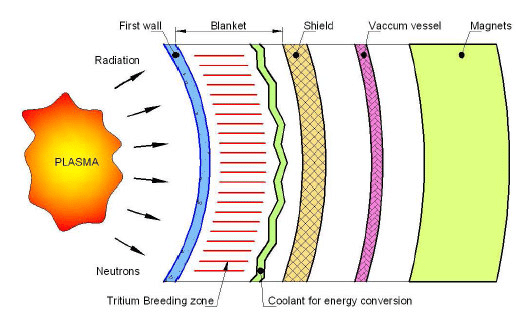
\includegraphics[width=0.7\linewidth]{Wall-Structure.png}
	\caption[Wall Structure for Tokamaks]{Wall structure for tokamaks. The "double-walled" structure in tokamaks often means the first wall and the vessel wall, along with layers between them.}
	\label{fig:wallstructure}
\end{figure}

At the heart of a working tokamak, the fusion plasma must reach temperatures of at least 100 million degrees Celsius. The first wall, as the innermost layer directly exposed to the plasma, must withstand extreme temperatures and high-energy particle bombardment \cite{abdou2015blanket}. To handle these conditions, materials such as beryllium, graphite, and tungsten are commonly employed \cite{wesson2011tokamaks,federici2001plasma,wilson1990beryllium,philipps2011tungsten}. Beryllium is valued for its low atomic number and high thermal conductivity, minimizing plasma contamination \cite{federici2001plasma,wilson1990beryllium}. Graphite offers excellent thermal shock resistance and mechanical stability at high temperatures \cite{federici2001plasma,wilson1990beryllium,philipps2011tungsten}. Tungsten, with its exceptionally high melting point and low sputtering yield, is often used in the divertor region \cite{wesson2011tokamaks,federici2001plasma,wilson1990beryllium,philipps2011tungsten}. These materials ensure that the plasma-wall interface effectively manages heat and minimizes impurity generation.

The vacuum vessel and its wall form an additional wall surrounding the first wall, typically constructed from stainless steel \cite{wesson2011tokamaks,federici2001plasma,iter_website,abdou2015blanket}. This double-walled structure houses essential systems, such as liquid cooling for thermal regulation, divertors for removing hot particles and protecting the first wall, and blanket modules for tritium breeding and neutron moderation \cite{abdou2015blanket}. The vacuum vessel also provides a vacuum space for better heat insulation and plasma confinement, serving as a safety buffer and accommodating various devices \cite{wesson2011tokamaks}.

The outermost layer of a superconducting tokamak consists of superconducting coils made from niobium-titanium (NbTi) and niobium-tin (Nb3Sn) \cite{wesson2011tokamaks, pong2012worldwide}. When cooled below their critical temperatures, these materials exhibit zero electrical resistance, enabling them to carry large currents for magnetic confinement with minimal energy loss. Maintaining these superconducting magnets at cryogenic temperatures, typically between 4K and 4.4K, requires a cryostat and bath of liquid helium \cite{pong2012worldwide, wesson2011tokamaks}. The cryostat, along with the vacuum space, provides thermal insulation, ensuring the superconducting coils stay at the necessary low temperatures despite their proximity to the hot plasma \cite{doshi2011iter, pong2012worldwide}.

ITER \cite{pong2012worldwide} and EAST \cite{wan2005progress} are among the most well-known tokamaks in the world. ITER is focusing on demonstrating the feasibility of large-scale fusion power, and its design incorporates advanced technologies such as plasma monitoring and tritium breeding blankets to sustain the fusion fuel cycle. Meanwhile, EAST explore more on long-duration plasma control technique \cite{wan2005progress}. ITER applies beryllium on the first wall interface while EAST still use tungsten on first wall. However, recent discussions regarding ITER suggest the potential application of tungsten on the first wall \cite{iter_website}. On both of ITER and EAST, tungsten is applied on divertor. Both of their vacuum vessels are made by stainless steel while ITER's vessel also houses some extra blanket modules designed for tritium breeding and neutron moderation. As for the superconducting coils, ITER use NbTi on poloidal field and Nb3Sn on toroidal field \cite{pong2012worldwide}, cooling by helium bath around 4K. For EAST, both coils of toroidal field and poloidal field take NbTi as primary choice. While there are technical differences between ITER and EAST, both are designed to achieve successful and sustainable fusion, with no expected significant disparities in their outcomes.

\section{Wall Modeling}
As discussed in the Chapter \ref{chapter 2}, the ideal MHD model is an appropriate approximate model for fusion plasma. In temperatures higher than 100 million degrees Celsius, the plasma is fully ionized and can be accurately described as an ideal plasma with no resistivity and viscosity.

The numerical modelling of tokamaks has been the focus of numerous studies in the literature. Some of these works regard the tokamak wall, as perfect conductor. Todd \textit{et al.} focuses on analyzing the stability of plasma configurations in tokamaks using the ideal MHD within perfect conducting walls \cite{todd1979dependence}. Pustovitov \textit{et al.} provides a comprehensive analysis of disruption forces in tokamaks using ideal MHD and perfect conducting wall assumptions, with a particular focus on applications to ITER \cite{pustovitov2017computation}. These conditions have benefits. The perfect conducting wall boundary condition can help stabilize certain MHD. By assuming that the wall is perfectly conducting with no resistivity, it can reflect any magnetic field perturbations as we discussed in the chapter \ref{chapter 2}, effectively providing a stabilizing effect on the plasma. This boundary condition simplifies the mathematical analysis and numerical implementation. These models are valuable for qualitative studies of the interactions between plasma and reactor walls.

In practice, no material exhibits perfect conductivity; even the most advanced superconductors possess inherent limitations. Modeling the wall as a perfect conductor ignores the actual electrical resistivity of materials used in tokamak walls. Most of the materials used on tokamak walls have finite resistivity. Ignoring the resistivities on these materials may lead to neglect on energy dissipation or magnetic field diffusion and the possibility of plasma instability \cite{pustovitov2017computation}. Generally, a perfect conducting condition simplify mathematical analysis but ignore resistive effects \cite{bondeson2003physics}. For more accurate results, modeling the tokamak wall as a perfect conductor is somewhat idealistic.

Modeling the tokamak walls as resistive walls is a more realistic approach. The materials, such as beryllium, graphite, or tungsten on the first wall and stainless steel on the vacuum vessel wall, are better described as resistive materials. Several studies have considered the effects of resistive walls, noting that their resistivities can lead to magnetic field diffusion and impact plasma behavior \cite{chrysanthou2020, ferraro2016multi, becerra2016resistive}. Over time, some magnetic fields may penetrate the wall, a phenomenon known as resistive wall mode (RWM), which may result in plasma instability \cite{clauser2021iter,bondeson2003physics}. Generally, resistive wall is a more realistic boundary condition under the scenario in a tokamak.

The following chapters, starting with chapter \ref{chapter 7}, will explore the theoretical foundations of resistive wall boundary conditions. In chapter \ref{chapter 8}, we will present a series of validation tests to compare the results of resistive wall conditions with those of a perfect conducting wall, demonstrating the impact on plasma behavior, further then apply these validated methods to a simulation within a tokamak-shaped vessel, illustrating the practical implications of our model. The report will conclude in chapter \ref{chapter 10} with a discussion on strategies for improving the accuracy of boundary conditions in future research.

 

 
